\chapter{Tight Binding method}
\label{ch:theory}
\section{Introduction to the tight-binding model} \label{sec:TB_theory}
Tight-binding method is developed to describe band structure of various materials, where electrons are localized at the atomic positions (tight-bonded to the atoms). In TB model simple effective Hamiltonian is used in contrast to first-principle calculations. 

Hear I provide short sketch of secular equation derivation.

The most essential approximation in TB model is the so-called two-center approximation, where Hamiltonian is approximated by the atomic Hamiltonian centered on the atomic positions in the unit cell $\vec{R}$ and only two-centered integrals are encountered.

Crystalline solids have translational symmetry along the directions of lattice vectors $a_i$. In further chapters I investigate both regular bulk materials, which have translational symmetry in three dimensions and nanomaterials, which have reduced symmetry. Translational symmetry enforces Bloch's theorem to be satisfied by solids' wave functions:
\begin{equation} \label{eq:blochs_theorem}
	\hat{T}_i \psi(\vec{k},\vec{r}) = \me^{i \vec{k} \cdot \vec{a_i}} \psi(\vec{k}\vec{r}),
\end{equation}
where $\hat{T}_i$ is the translational operator along the lattice vector $\vec{a_i}$ and $\vec{k}$ is the Bloch wave vector \cite{kittel}.

We construct the Bloch wave function of the crystal as a linear combination of the local Wannier functions, which are approximated by the eigenfunctions of the atomic Hamiltonian, the atomic orbitals $\phi_{i}(\vec{r} - \vec{t_i} - \vec{R_j})$, where $\vec{t_i}$ is the position of atom in the unit cell at cite $\vec{R_j}$, $i$ is a set of quantum numbers identifying the type of orbital: $n$, $l$, $m$ -- the principal, angular-momentum and magnetic quantum numbers, respectively and $s$ -- spin. The Bloch wave function looks as follows:
\begin{equation} \label{eq:wave_fun}
	\psi_{j}(\vec{k},\vec{r}) = \frac{1}{\sqrt{N}} \sum_{\vec{R_j}} \me^{i\vec{k}(\vec{R_j} + \vec{t_i})} \phi_{i} (\vec{r} - \vec{t_i} - \vec{R_j}),
\end{equation}
where N is the number of unit cells in the crystal. It's easy to see that constructed in such a way wave function satisfies Bloch's theorem (eq. \ref{eq:blochs_theorem}).

Hamiltonian's eigenfunctions $\Psi_j(\vec{k}, \vec{r})$ are defined as a linear combination of Bloch functions:
\begin{equation} \label{eq:wave_function_expansion}
	\Psi_j(\vec{k}, \vec{r}) = \sum_{j'=1}^{n} C_{jj'}(\vec{k}) \psi_j(\vec{k}, \vec{r})
\end{equation}

Energies of the system characterized by Hamiltonian $\hat{H}$ are given by
\begin{equation}
	E_i(\vec{k}) = \frac{\langle \Psi_i | \hat{H} | \Psi_i \rangle}{\langle \Psi_i | \Psi_i \rangle} = \frac{\int \Psi^*_i(\vec{k}, \vec{r}) \hat{H} \Psi_i(\vec{k}, \vec{r}) dr}{\int \Psi^*_i(\vec{k}, \vec{r}) \Psi_i(\vec{k}, \vec{r}) dr}
\end{equation}
Expantion of $\Psi_j(\vec{k}, \vec{r})$ according to eq. \ref{eq:wave_function_expansion} leads to
\begin{equation}
	E_i(\vec{k}) = \frac{\sum\limits_{j,j'=1}^{n} C^*_{ij} C_{ij'} \langle \psi_j | \hat{H} | \psi_{j'} \rangle}{\sum\limits_{j,j'=1}^{n} C^*_{ij} C_{ij'} \langle \psi_j | \psi_{j'} \rangle} = \frac{\sum\limits_{j,j'=1}^{n} H_{jj'}(\vec{k}) C^*_{ij} C_{ij'}}{\sum\limits_{j,j'=1}^{n} S_{jj'} C^*_{ij} C_{ij'}},
\end{equation} 
where $H_{jj'}(\vec{k})$ and $S_{jj'}(\vec{k})$ are Hamiltonian (transfer) and overlap matrices elements, respectively, and are defined by
\begin{equation} \label{eq:h_matrix}
	H_{jj'}(\vec{k}) = \langle \psi_j | \hat{H} | \psi_{j'} \rangle
\end{equation}
\begin{equation} \label{eq:s_matrix}
	S_{jj'}(\vec{k}) = \langle \psi_j | \psi_{j'} \rangle
\end{equation}
For a given $\vec{k}$ value, coefficient $C^*_{ij}(\vec{k})$ is optimized to minimize $E_i(\vec{k})$:
\begin{equation}
	\frac{\partial E_i (\vec{k})}{\partial C^*_{ij}} = \frac{\sum\limits_{j'=1}^{n} H_{jj'}(\vec{k}) C_{ij'}}{\sum\limits_{j,j'=1}^{n} S_{jj'} C^*_{ij} C_{ij'}} - \frac{\sum\limits_{j,j'=1}^{n} H_{jj'} C^*_{ij} C_{ij'}}{[\sum\limits_{j,j'=1}^{n} S_{jj'} C^*_{ij} C_{ij'}]^2} \sum\limits_{j'=1}^{n} S_{jj'}(\vec{k}) C_{ij'}(\vec{k}) = 0.
\end{equation}
This can be simplified as 
\begin{equation}
	\sum_{j'=1}^{n} H_{jj'}(\vec{k}) C_{ij'}(\vec{k}) - E_i(\vec{k}) \sum_{j'=1}^{n} S_{jj'}(\vec{k}) C_{ij'}(\vec{k}) = 0
\end{equation}
or in the matrix form:
\begin{equation} \label{eq:secular}
	(\overline{\overline{H}} - E_i(\vec{k})\overline{\overline{S}})\overline{C_i}(\vec{k}) = 0
\end{equation}

Usually integration results are taken as parameters, which have to be fitted to reproduce certain solid's properties or the band structure calculated by first-principle approach. Matrix Elements in \ref{eq:h_matrix} and \ref{eq:s_matrix} where $\vec{R} = \vec{R'}$ are called on-site elements, and for $\vec{R} \neq \vec{R'}$ they are called hopping and overlap parameters respectively. 

In general case, atomic orbitals centered on different sites are not orthogonal and the corresponding overlap parameters have small but finite values.But often orthogonal basis of orbitals is used, so that overlap matrix becomes identity matrix and energies are eigenvalues of the Hamiltonian matrix. In the following sections I will discuss both approaches. 

The next approximation is to consider a finite as small as necessary number of orbitals per atom. The number of solutions of the secular equation in \ref{eq:secular} is equal to dimension of the Hamiltonian matrix,
\begin{equation}
dim = g \times \sum_j n_j
\end{equation}
Here $g$ is spin factor ($1$ or $2$), summation goes through all atoms in unit cell and $n_j$ is number of included orbitals for atom $j$.

In the final nearest neighbors approximation (NNA) only the nearest neighbors of a chosen atom are taken into account in the Hamiltonian and overlap matrix elements eqs. (\ref{eq:h_matrix}) and (\ref{eq:s_matrix}).
\section{Vanishing and Non-vanishing Orbital Interactions Based on TB model}
To solve the eigenvalue problem (eq. \ref{eq:secular}) one needs to calculate Hamiltonian and overlap matrices elements between atomic orbitals at different locations. In this work I use so-called rotating atomic orbitals $\phi_{lm}$ which are characterized by the angular momentum $l = {s, p, d, ...}$ and the magnetic quantum number $m$. Due to the spherical symmetry of the atomic potential the orbital function may be separated in the radial part and angular part:
\begin{equation}
	\phi_{lm}(\vec{r}) = R_l(\vec{r}) Y_m(\theta, \phi)
\end{equation}
The angular part is described by spherical harmonics:
\begin{equation}
	Y_{l,m}(\theta, \phi) = (-1)^m \sqrt{\frac{(2l + 1)(l-m)!}{4 \pi (l+m)!}} P_l^m(\cos{\theta})\me^{i m \phi}
\end{equation}
The hopping and overlap integrals between those atomic orbitals, which are localized on the atoms at the positions $\vec{R}$ and $\vec{R'}$,
\begin{equation}
	V_{ll'|m|} \delta_{mm'}\langle l', m', \vec{R'} | \hat{H} | l, m , \vec{R} \rangle
\end{equation}
\begin{equation}
	S_{ll'|m|} \delta_{mm'}\langle l', m', \vec{R'} | l, m , \vec{R} \rangle
\end{equation}
are called Slater-Koster (SK) parameters \cite{slatter}. If the relative vector $\vec{R}-\vec{R'}$ is parallel to the quantization axes of the orbitals $\phi_{l,m}(\vec{r} - \vec{R}) = \langle \vec{r} | l, m, \vec{R} \rangle$. The SK parameters are diagonal in the magnetic number $m$. Each value of $m$ is related to the different kind of bonding given by the superpositions the atomic orbital wave functions. The different bonding types are denoted by the Greek letters $\sigma$, $\pi$, $\delta$, which correspond to the magnetic numbers $m = {0, 1, 2}$, respectively, and are related to the homonymous molecular orbitals, which are shown schematically in \ref{fig:orbitals}. 
\begin{figure}[hb]  \label{fig:orbitals}
  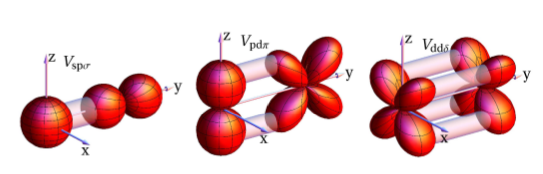
\includegraphics[width=\linewidth]{img/orbitals}
  \caption[caption]{Sketch of SK hopping parameters $V_{sp\sigma}$, $V_{pd\pi}$ and $V_{dd\delta}$ that represent different kinds of bonding $\sigma$, $\pi$ and $\delta$, respectively, shown by the tunnels between the two orbital states\footnotemark}
\end{figure}
\footnotetext{http://epub.uni-regensburg.de/22863/4/PhDthesis.pdf}

For arbitrary vector $\vec{R} - \vec{R'} $ the hopping $\langle l', m', \vec{R'} | \hat{H} | l,m,\vec{R} \rangle$ and overlap $\langle l', m', \vec{R'} | l,m,\vec{R} \rangle$ integrals are given by linear combinations of the SK parameters. 

\begin{figure}[h]  \label{fig:sp}
  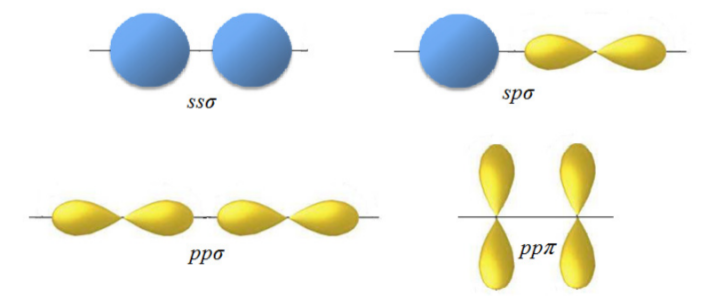
\includegraphics[width=\linewidth]{img/sp_bonding}
  \caption[caption]{sp-bonding correspond to non-vanishing matrix elements.\footnotemark}
\end{figure}
\footnotetext{http://sina.sharif.edu/~khorasani/Publications/Graphene.pdf}
\begin{figure}[h]  \label{fig:sp_vanishing}
  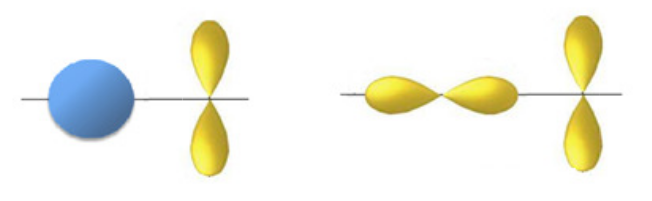
\includegraphics[width=\linewidth]{img/sp_vanishing}
  \caption[caption]{sp-bonding correspond to vanishing matrix elements.\footnotemark}
\end{figure}
\footnotetext{http://sina.sharif.edu/~khorasani/Publications/Graphene.pdf}

To reduce the number of the corresponding hopping and overlap parameters one can exploit the symmetries of the atomic orbitals. For example, in case bonding including $s$ and $p$ orbitals, there are only four non-zero overlapping integrals, as shown schematically on fig. \ref{fig:sp}. The remaining cases like those shown on fig. \ref{fig:sp_vanishing} correspond to the matrix elements which vanish because of symmetry constraints. In general the $p$ orbitals are not just parallel or lie on the line that joins the atomic positions. We can always project each $p$ orbital into two components, one of them along the bonding line, the other one perpendicular to it. 

The general form of hopping integrals withing the $s$, $p$ and $d$ orbitals is presented in table \ref{tab:hopping_integrals}. In this table $n_x$, $n_y$ and $n_z$ are Cartesian components of unit vector, connecting two orbitals:
\begin{equation}
	\vec{n} = \frac{\vec{R} - \vec{R'}}{|\vec{R} - \vec{R'}|},
\end{equation}
which are related to Euler angles as follows:
\begin{equation}
	n_x =\cos{\alpha} \sin{\beta}, n_y = \sin{\alpha} \sin{\beta}, n_z = \cos{\beta}. 
\end{equation}

The overlap of two displaced directed orbitals has exactly the same structure, where the SK hopping parameters $V_{l l' |m|}$ have to be replaced by the overlap parameters $S_{l l' |m|}$. Using the hopping parameters in table \ref{tab:hopping_integrals} one is able to construct the multi-orbital TB Hamiltonian to model the band structure of desired material.

\begin{table}[h!]
\begin{center}
\begin{tabularht}{0.9\textheight}{|l| l|}
\hline
% \textbf{Parametr} & \textbf{6H-SiC} & \textbf{4H-SiC}\\ \hline
 \interrowfill
$\langle s | \hat{H} | s \rangle $ & $V_{ss \sigma}$ \\ \interrowfill
$\langle s | \hat{H} | p_i \rangle $ & $n_i V_{sp \sigma}$ \\ \interrowfill
$\langle s | \hat{H} | d_{ij} \rangle $  & $\sqrt{3} n_i n_j V_{sd\sigma}$  \\ \interrowfill
$\langle s | \hat{H} | d_{x^2 - y^2} \rangle $& $\frac{\sqrt{3}}{2} (n_x^2 - n_y^2) V_{sd\sigma}$\\ \interrowfill
$\langle s | \hat{H} | d_{z^2} \rangle $ & $-\frac{1}{2}(n_x^2 + n_y^2 - 2n_z^2) V_{sd\sigma} $\\ \interrowfill
$\langle p_i | \hat{H} | p_i \rangle $ & $n_i^2 V_{pp\sigma} + (1 - n_i^2) V_{pp\pi}$\\\interrowfill
$\langle p_i | \hat{H} | p_j \rangle $ & $-n_i n_j (V_{pp \pi} - V_{pp \sigma}) $ \\ \interrowfill
$\langle p_i | \hat{H} | d_{ij} \rangle $ & $\sqrt{3}n_i^2 n_j V_{pd\sigma} (1 - 2 n_i^2) n_j V_{pd\pi} $ \\\interrowfill
$\langle p_i | \hat{H} | d_{jk} \rangle $ & $n_x n_y n_z (\sqrt{3} V_{pd\sigma} - 2 V_{pd\pi}) $ \\ \interrowfill
$\langle p_x | \hat{H} | d_{x^2 - y^2} \rangle $ & $\frac{\sqrt{3}}{2}n_x(n_x^2 - n_y^2) V_{pd\sigma} + n_x (1-n_x^2 + n_y^2) V_{pd\pi} $ \\\interrowfill
$\langle p_y | \hat{H} | d_{x^2 - y^2} \rangle $ & $\frac{\sqrt{3}}{2}n_y(n_x^2 - n_y^2) V_{pd\sigma} - n_y (1-n_y^2 + n_x^2) V_{pd\pi} $ \\ \interrowfill
$\langle p_z | \hat{H} | d_{x^2 - y^2} \rangle $ & $\frac{\sqrt{3}}{2}n_z(n_x^2 - n_y^2) V_{pd\sigma} - n_z (n_x^2 + n_y^2) V_{pd\pi} $ \\  \interrowfill
$\langle p_i | \hat{H} | d_{z^2} \rangle $ & $-\sqrt{3} n_z (n_x^2 + n_y^2) V_{pd\pi} - \frac{1}{2} n_z (n_x^2 + n_y^2 - 2n_z^2) V_{pd\sigma} $ \\  \interrowfill
$\langle p_z | \hat{H} | d_{z^2} \rangle $ & $\sqrt{3}n_z(n_x^2 + n_y^2)V_{pd\pi} - \frac{1}{2} n_z (n_x^2 + n_y^2 - 2n_z^2)V_{pd\sigma} $ \\  \interrowfill
$\langle d_{ij} | \hat{H} | d_{ij} \rangle $ & $n_i^2 n_j^2 (3V_{dd\sigma} - 4 V_{dd\pi} + V_{dd\pi}) + (n_i^2 + n_j^2)V_{dd\pi} + n_k^2 V_{dd\delta} $ \\ \interrowfill
$\langle d_{ij} | \hat{H} | d_{ik} \rangle $ & $n_i^2 n_j n_k(3V_{dd\sigma} - 4 V_{dd\pi} + V_{dd\pi}) + n_j n_k (V_{dd\pi} - V_{dd\delta}) $ \\  \interrowfill
$\langle d_{xz} | \hat{H} | d_{x^2 - y^2} \rangle $ & $\frac{1}{2} n_x n_z ((n_x^2 - n_y^2)(3V_{dd\sigma} - 4V_{dd\pi} + V_{dd\delta}) + 2(V_{dd\pi} - V_{dd\delta})) $ \\  \interrowfill
$\langle d_{yz} | \hat{H} | d_{x^2 - y^2} \rangle $ & $\frac{1}{2} n_y n_z ((n_x^2 - n_y^2)(3V_{dd\sigma} - 4V_{dd\pi} + V_{dd\delta}) - 2(V_{dd\pi} - V_{dd\delta})) $ \\  \interrowfill
$\langle d_{xy} | \hat{H} | d_{x^2 - y^2} \rangle $ & $\frac{1}{2} n_x n_y (n_x^2 - n_y^2)(3V_{dd\sigma} - 4V_{dd\pi} + V_{dd\delta}) $ \\  \interrowfill
$\langle d_{xz} | \hat{H} | d_{z^2} \rangle $ & $-\frac{\sqrt{3}}{2} n_x n_z ((n_x^2 + n_y^2)(V_{dd\sigma} - 2V_{dd\pi} + V_{dd\delta})  + 2n_z^2(V_{dd\pi} - V_{dd\sigma})) $ \\  \interrowfill
$\langle d_{yz} | \hat{H} | d_{z^2} \rangle $ & $-\frac{\sqrt{3}}{2} n_y n_z ((n_x^2 + n_y^2)(V_{dd\sigma} - 2V_{dd\pi} + V_{dd\delta})  + 2n_z^2(V_{dd\pi} - V_{dd\sigma}))$ \\  \interrowfill
$\langle d_{xy} | \hat{H} | d_{z^2} \rangle $ & $\frac{\sqrt{3}}{2} n_y n_z (n_z^2(3V_{dd\sigma} - 4V_{dd\pi} + V_{dd\delta}) + V_{dd\delta} - V_{dd\sigma}) $ \\ \interrowfill
$\langle d_{x^2-y^2} | \hat{H} | d_{z^2} \rangle $ & $\frac{1}{4} (n_x^2 - n_y^2) (n_z^2(3V_{dd\sigma} - 4V_{dd\pi} + V_{dd\delta}) + V_{dd\delta} - V_{dd\sigma}) $ \\ \interrowfill
$\langle d_{x^2-y^2} | \hat{H} | d_{x^2-y^2} \rangle $ & $\frac{1}{4} (n_x^2 - n_y^2)^2 (3V_{dd\sigma} - 4V_{dd\pi} + V_{dd\delta}) + (n_x^2 + n_y^2) V_{dd\pi}  + n_z^2 V_{dd\delta} $ \\ \interrowfill
$\langle d_{z^2} | \hat{H} | d_z^2 \rangle $ & $\frac{3}{4} (n_x^2 + n_y^2)^2 V_{dd\delta} + 3(n_x^2 + n_y^2) n_z^2 V_{dd\pi} + \frac{1}{4}(n_x^2 + n_y^2 - 2n_z^2)^2 V_{dd\sigma} $ \\ \interrowfill
\hline
\end{tabularht}
\end{center}
\caption{The hopping integral within the directed orbitals with the maximum angular momentum $l = 2$. Here I use the indexes $i = {x, y, z}$, $j = {x, y, z}$, $k = {x, y, z}$ with the rule $i = j = k$. The complex conjugated hopping integrals are given by $\langle l | \hat{H} | l' \rangle = (-1)^{l+l'} \langle l' | \hat{H} | l \rangle$.}
\label{tab:hopping_integrals}
\end{table}

\section{Spin-orbit interaction}
Spin itself and it's coupling with orbital motion of the electrons are relativistic effects, which can be derived from Dirac equation. In the non-relativistic limit spin-orbit coupling (SOC) can be taken into account as an additional term in the Hamiltonian given by
\begin{equation} \label{eq:soc0}
	\hat{H}^{SO} = \frac{1}{2 m^2 c^2} (\vec{\nabla} \times \vec{p}) \cdot \vec{S},
\end{equation}
where $m$ is electron mass, $c$ the speed of light, $\vec{p}$ momentum and $\vec{S} = \frac{}{2} \vec{s}$ is the spin operator. Components of spin operator are Pauli matrices $\sigma_i$, $i = \{x, y, z\}$.

SOC term in eq. \ref{eq:soc0} looks like Zeeman term for electron in effective magnetic field $\vec{B}_{eff} = \frac{\vec{\nabla} \times \vec{p}}{m c^2}$. In TB model potential $V(\vec{r})$ is approximated by spherically symmetric potential (see section \ref{sec:TB_theory}). So that $V(\vec{r}) = V(|\vec{r}|)$ and $\vec{\nabla} V = \frac{\vec{r}}{r} \frac{dV}{dr}$. Here I will consider on-site contribution to the TB Hamiltonian. Such approximation is legal because major SOC effect comes from the orbits close to the atomic nuclei \cite{soc}. In this approximation the SOC operator can be rewritten as a term which couples the spin and angular momentum: 
\begin{equation} \label{eq:hsoc}
	\hat{H}^{SO} =  \xi(\vec{r}) \vec{L} \cdot \vec{S},
\end{equation}
where where the function $\xi(\vec{r})$ contains the entire radial dependence of the SOC Hamiltonian.

Scalar product of angular momentum and spin in eq. \ref{eq:hsoc} can be presented in terms of ladder operators:
\begin{equation}
	\vec{L} \cdot \vec{S} = \frac{1}{2} (\hat{L}_{+} \hat{S}_{-} + \hat{L}_{-} \hat{S}_{+}) + \hat{L}_z \hat{S}_z,
\end{equation}
where
\begin{equation}
	\hat{L}_{\pm} = \hat{L}_{+} \pm i\hat{L}_{-},\qquad \hat{S}_{\pm} = \hat{S}_{+} \pm i\hat{S}_{-}.
\end{equation}
Ladder angular momentum operators act on atomic orbital wave functions as follows:
\begin{equation}
	\hat{L}_{\pm} |l, m \rangle = \sqrt{l(l+1) - m (m \pm 1)} |l, m \pm 1 \rangle, \qquad \hat{L}_z |l, m \rangle = m |l, m \rangle
\end{equation}
Finally using the orthogonality of atomic orbitals we obtain a set of non-zero on-site expectation values of the SOC Hamiltonian:
\begin{equation}
 	\langle l,m, \vec{R} | \hat{H^{SO}} | l', m', \vec{R} \rangle = \xi_l \delta_{l,l'} \langle l, m | \vec{L} \cdot \vec{S} | l', m' \rangle,
\end{equation} 
where the strength of the atomic SOC $\xi_l$ (frequently denoted also as $\lambda_l$) is given by 
\begin{equation}
	\xi_l = \int\limits^\infty_0 dr R^2_l(r) \xi(r)
\end{equation}
must be fitted to reproduce the SOC effects in the band structure obtained by the first principal calculations or experimental data.The on-site matrix elements of the dimensionless part of the SOC Hamiltonian $\vec{L} \cot \vec{S} $ in the bases of the rotating orbitals are placed in the table \ref{tab:soc1} and in the basis of directed orbitals (which will be used further in this work) -- in table \ref{tab:soc2}.

\begin{table}[h!]
\begin{tabularx}{\textwidth}{|r| X X X X|}
\hline
orbital & $|0, 0 \rangle$ & $|1, -1 \rangle$ & $|1, 0 \rangle$ & $|1, 1 \rangle$ \\ \hline
$\langle 0, 0|$ & 0 & 0 & 0 & 0 \\
$\langle 1, -1|$ & 0 & $-s_z$ & $\frac{1}{\sqrt{2}} s_{+} $ & 0 \\
$\langle 1, 0|$ & 0 & $\frac{1}{\sqrt{2}} s_{-} $ & 0 & $\frac{1}{\sqrt{2}} s_{+} $ \\
$\langle 1, -1|$ & 0 & 0 & $\frac{1}{\sqrt{2}} s_{-} $ & $s_z$ \\ \hline
\end{tabularx}
\newline
\vspace*{0.5 cm}
\newline
\begin{tabularx}{\textwidth}{|r| X X X X X|}
\hline
orbital & $|2, -2 \rangle$ & $|2, -1 \rangle$ & $|1, 0 \rangle$ & $|2, 1 \rangle$ & $|2, 2 \rangle $ \\ \hline
$\langle 2, -2|$ & $-2 s_z$ & $s_{+} $ & 0 & 0 & 0\\
$\langle 2, -1|$ & $s_{-}$ & $-s_z$ & $\sqrt{\frac{3}{2}} s_{+} $ & 0 & 0\\
$\langle 2, 0|$ & 0 & $\sqrt{\frac{3}{2}} s_{-} $ & 0 & $\sqrt{\frac{3}{2}} s_{+} $ & 0\\
$\langle 2, 1|$ & 0 & 0 & $\sqrt{\frac{3}{2}} s_{-} $ & $s_z$ & $s_{+} $\\
$\langle 2, 2|$ & 0 & 0 & 0 & $s_{-} $ & $2 s_z $\\
\hline
\end{tabularx}
\caption{Matrix elements of the SOC operator $\vec{L} \cdot \vec{s}$ in the basis of rotating orbitals.}
\label{tab:soc1}
\end{table}

\begin{table}[h!]
\begin{tabularx}{\textwidth}{|r| X X X X|}
\hline
orbital & $|s \rangle$ & $|p_x \rangle$ & $|p_y \rangle$ & $|p_z \rangle$ \\ \hline
$\langle s|$ & 0 & 0 & 0 & 0 \\
$\langle p_x|$ & 0 & 0 & $- i s_z$ & $i s_y$ \\
$\langle p_y|$ & 0 & $i s_{z} $ & 0 & $- i s_{x} $ \\
$\langle p_z|$ & 0 & $-i s_y$ & $i s_{x} $ & $s_z$ \\
\hline
\end{tabularx}
\newline
\vspace*{0.5 cm}
\newline
\begin{tabularx}{\textwidth}{|r| X X X X X|}
\hline
orbital & $|d_{xy} \rangle$ & $|d_{x^2-y^2}	\rangle$ & $|d_{xz} \rangle$ & $|d_{yz} \rangle$ & $|d_{z^2} \rangle $ \\ \hline
$\langle d_{xy}|$ & 0 & $2 i s_z $ & $-i s_x $ & $i s_y$ & 0\\
$\langle d_{x^2 - y^2}|$ & $-2 i s_z$ & $0$ & $i s_{y} $ & $i s_x $ & 0\\
$\langle d_{xz}|$ & $i s_x$ & $- i s_{y} $ & 0 & $-i s_{z} $ & $i \sqrt{3} s_y$\\
$\langle d_{yz}|$ & $- i s_y $ & $ - i s_x$ & $i s_{z} $ & $0$ & $-i \sqrt{3} s_x $\\
$\langle d_{z^2}|$ & 0 & 0 & - $i \sqrt{3} s_y$ & $i \sqrt{3} s_{x} $ & $0$\\
\hline
\end{tabularx}
\caption{Matrix elements of the SOC operator $\vec{L} \cdot \vec{s}$ in the basis of rotating orbitals.}
\label{tab:soc2}
\end{table}